%% Author: Sakhile Masoka (851667@students.wits.ac.za)
%% Homepage: https://github.com/smasoka/CODE-RADE-project/tree/sakhile-project
%% Reference: 
\RequirePackage{ifpdf}
\documentclass [titlepage,11pt]{article}

\usepackage{graphicx}
\usepackage{witsa4}
\usepackage{times}
\usepackage{enumerate}
\usepackage[inline]{enumitem}

\usepackage{url}
\usepackage{natbib}

\usepackage[center]{titlesec}

% Force natbib.sty to put citation labels in the reference list
\makeatletter
\renewcommand\NAT@biblabel[1]{\def\citeauthoryear##1##2{##1 ##2}[#1]\hfill}
\renewcommand\NAT@bibsetup[1]{%
  \setlength{\itemsep}{\bibsep}\setlength{\parsep}{\z@}}
\def\@lbibitem[#1]#2{%
  \if\relax\@extra@b@citeb\relax\else
    \@ifundefined{br@#2\@extra@b@citeb}{}{%
     \@namedef{br@#2}{\@nameuse{br@#2\@extra@b@citeb}}}\fi
   \@ifundefined{b@#2\@extra@b@citeb}{\def\NAT@num{}}{\NAT@parse{#2}}%
   \item[\hfil\hyper@natanchorstart{#2\@extra@b@citeb}\@biblabel{#1}%
    \hyper@natanchorend]%
    \NAT@ifcmd#1(@)(@)\@nil{#2}}
\makeatother
\bibliographystyle{named-wits}
\bibpunct{[}{]}{;}{a}{}{}


\title{\Huge Continuous Delivery of Research Application in a Distributed Environment \\\medskip Research Proposal}
\author{Sakhile Masoka (851667@students.wits.ac.za)\\Witwatersrand University}

\begin{document}
\maketitle



% Provides Context
% Idea Of Own Contribution
% What Will Be Done
% How It Will Be Done
% Can Be Read Independently
% Measures (metrics) Used and Results Very Good
\begin{abstract}
One of the aims of e-Infrastructures is to provide easy access to powerful computational and data platforms, to as many eligible users as possible. The South African National Grid (SAGrid), as part of the National Integrated Cyberinfrastructure System is no exception. While access to the users is being simplified greatly by the adoption of science gateways and identity federations, the community of application developers and technical support in scientific collaborations does not yet have an easy way to integrate these applications in the first place.\\

SAGrid has identified this as a gap in the services it provides and has developed a solution to
the issue of easily integrating new applications into the infrastructure in a fast, flexible, distributed and reproducible way. Using existing tools and services, SAGrid has defined a simple set of tests which applications need to pass in order to be considered valid for the infrastructure.\\  

The proposal is to use a continuous integration platform, Jenkins, to encode these tests automatically. Critical to the process is the Inter-operability between source code repository, automated build system, artifact creation and a content delivery system to sustain the system. These will be tested using scientific applications, namely GADGET, Quantum Espresso and python based application framework such as R. The tests will be executed in bash scripts to applications that subscribes to CVMFS repositories.

\end{abstract}


\tableofcontents{}


% Introduces General Problem Area
% Introduces Specific Problem Area
% Research To Be Followed
% Provides Idea About Expected Results
% Provides Idea Of Research Contribution
% Correct Level Of Detail? 
% Provides Structure to Rest Of Document

% One of the aims of e-Infrastructures is to provide easy access to powerful computational and data
% platforms, to as many eligible users as possible. The South African National Grid (SAGrid), as part
% of the National Integrated Cyberinfrastructure System is no exception. While access to the users is
% being simplified greatly by the adoption of science gateways and identity federations, the community
% of application developers and technical support in scientific collaborations does not yet have an easy
% way to integrate these applications in the first place.
\section{Introduction}

e-Science  is computationally intensive science that is carried out in highly distributed network environments, or science that uses immense data sets that require grid computing, the term sometimes includes technologies that enables distributed collaboration, such as the Access Grid. \citep{escience}. This leads to working definition of e-Infrastructures as networked tools, data and resources that support a community of researchers, broadly including all those who participate in and benefit from research. e-Infrastructures include services as diverse as the physical supply of backbone connectivity,single- or multi-purpose grids, supercomputer infrastructure, data grids and repositories, tools for visualization, simulation, data management, storage, analysis and collection, tools for
support in relation to methods or analysis, as well as remote access to research instruments and very large research facilities, according to the eResearch2020 Final Report \citep{eresearch}.\\ 

The National Integrated Cyberinfrastructure System (NICIS) is a framework of an integrated system for cyberinfrastructure in South Africa, which includes pillars of data, computations and network infrastructure. South African Grid (SAGrid) is part of the South African National Research Network (SANReN), which in-turn is one of the network pillars on NICIS. SAGrid carries the mandate to enable anyone, with the right credentials to access the Cyberinfrastructure (data,compute,software,metadata, support, etc services) and to provide tools for collaboration and research \citep{nicis}. \\

% The General/Specific Problem and Solution
In this mandate, access to the users is being simplified greatly by the adoption of science gateways and identity federations, but the community of application developers and technical support in scientific collaborations does not yet have an easy way to integrate these applications. SAGrid has defined tests which applications need to pass in order to be considered valid for the infrastructure and using existing tools and services, these tests can be automated using continuous integration platforms. This research proposal aims to look at the methodologies and the platforms tools to encode these test as automated. The results will lead to insights necessary to provide best-practice guidelines to future development and operation of the service, especially related to optimisation and automation procedures.\\

% Structure of the paper
The paper is structured as follows:Section 2 describes the problem statement, motivation and literature review. Section 3 looks into the research aim, discussing the research aims to answer. Section 4 describes the research methodology, the software's and actual work to be done. Section 5 discusses the results and lastly section 6 is the conclusion. \\

% Provides Detail On Specific Problem Area
% Level Of Engagement With Research Literature
% Level Of Understanding Of Problem Background
% Contains Adequate And Relevant References 
% Contains Relevant Ideas, Concepts, etc., From References
% Relates Background Material And Related Work To Research Question
% Research Aim/Question Justified In Terms Of Past Research

% SAGrid has identified this as a gap in the services it provides and has developed a solution to
% the issue of easily integrating new applications into the infrastructure 
% in a fast, flexible, distributed and reproducible way.
\section{Background}

% Detail description of the problem statement
\subsection{Problem Statement and Motivation}

% Explain how the applications are installed? 
Grid applications usually are installed by sending jobs to Grid sites. The jobs contain instructions to install and configure applications. Once applications are installed, site administrators are notified and they flag the site, informing the general public of the availability of the application. This process has some flaws, one being sites are configured differently, one installation in another site is not guaranteed to work on another. This is caused by different configured variables, different configured paths, dependencies, compatibility with different versions etc. This calls for the application scientist to know a great deal about the infrastructure when the application is being installed. Since application scientist are not site administrators, this becomes a big problem. To name the issues faced with this approach in a number format, 1. Applications are not centrally managed. 2. Dependency complications 3. For each step, failure, manual intervention is needed by either the application scientist or the site administrator. \\

Solving one of these problems leads to solving the next, for example once applications are managed centrally, solving dependency complexity and version control will be easy, infact it inherent to managing applications centrally. Managing applications centrally also makes site secure. Not every user can send jobs to install or be malicious. Site administrators can configure secure permissions without worrying about if a certain job is an installation or not. Solving dependency complexity by packaging every needed component in each an every installation makes deployment platform independent. Meaning, one installation will work on every site. To properly makes make this solution work, a remote repository which site infrastructures subscribe to makes deployment easy and manageable. On the repository, either an installed application is available for execution or installation files are available for installation that will not fail. This depends on caching blah blah blah....  \\

Motivation: Integration, Fast, Flexible and reproducible (DevOps). 
The proposed solution is integrated, from application development to application deployment, all steps are linked together. Its fast, all steps are combined together, eliminating duplication of work, access communications and allows administrators either site or application to focus on their work, not overlapping. Flexible in sense that firstly it scales, secondly its adaptable to all grid communities and thirdly, changes in site infrastructures has little affect on deployment, at worse a re-deployment is needed but no changes to the application is needed in-order for the application to work on the ``new'' site.  Lastly, using containers, the solution produces artefact's (installation files) which can be used anywhere. This solution is based on DevOps and CI philosophies. \\

% Literature Review on CODE-RADE
% I need to check my literature review on this, how to tailor it to this: Now. 
\subsection{Literature Review: }
Review on the approach \\
Review of the application software's to be used in the solution \\
Adapt the literature review to the proposal. \\

% Has Presented Research Hypothesis/Focused Research Question
% Has Clearly Stated Hypothesis/Research Question
% Hypothesis Can Be Tested And Research Question Can Be Answered

% The specific problems we aim to address in this limited-scope project are those of automation and
% distribution. Specifically How far is it feasible to automate the build steps in order to produce high-quality, 
% re-distributable artifacts ?
% How are dependencies of applications to be managed in various configurations ?
% How can Linux containers be used to distributed these artifacts to remote sites with the minimum
% intervention necessary by site administrators
\section{Research Aim}
The specific problems this project aims to address are those of automation and distribution with the following questions (and their descriptions).  \\
% A mention of Jenkins and Docker
\begin{description}

\item \textbf{How far is it feasible to automate the build steps in order to produce high-quality, re-distributable artifacts?} Can automating every build step results into producing high quality artifacts? Another question is, can all the build steps be automated or some manual testing will still be needed? For this question, the project will explore the pipeline of delivering a scientific application in a distributed infrastructure by looking into software development disciples namely \emph{Continuous Delivery} \cite{delivery15} and \emph{Continuous Integration} \citep{fowler06}. Both these disciples stem from DevOps \citep{wikiOps}, a software development method  stresses communication, collaboration, integration, automation, and measurement of cooperation between software developers. Specifically, Jenkins will be highlighted as the best software platform to possibly to explore, implement and answer this question. \\

\item \textbf{How are dependencies of applications to be managed in various configurations?} With different scientific applications having different degrees of complex dependencies, how can ``dependency hell''\citep{dependency} be solved? These degrees of complexity come in different forms like circular and conflicting dependencies or just a long list of dependencies which requires large download times and disk space. Some of these complexes arises from packages on the system being updated or upgraded and lastly, when compiling the same software application but with different options enabling further functionality e.g.\ enabling GPU support which requires cuda libraries. Using containers, specifically Docker, we'll discuss how this problem can be solved by wrapping the software application in a complete file-system that contains everything it needs to run: code, runtime, system tools, system libraries etc... which guarantees that it will always run the same, regardless of the environment it is running in \citep{dockerWeb}. \\

\item \textbf{How can Linux containers be used to distribute these artifacts to remote sites with the minimum intervention necessary by site administrators?} We want site administrators to remain site administrators, meaning they shouldn't be concern about what an application administrators or scientists are doing. These artifacts should be deployable by minimum efforts, and since they are independent, complete on their own, site administrators don't need to do anything except mount CVMFS repository that deliverers the artifacts. CVMFS (CernVM File System) is a network file system based on HTTP and optimized to deliver software in a fast, scalable, and reliable way \citep{jakob11}. SAGrid site infrastructures subscribe to this repository and that makes it feasible.  \\

\end{description}

% It Is presented
% It Appears To Be A Reasonable Approach
% It Will Lead To Verification Or Refutation Of Research Hypothesis
% It Will Lead To Answering Of The Research Question Adequate 
% Student Has Identified Data To Be Collected/Measurements To Be Made
% Student Has Motivated Why Data Or Measurements Have Been Selected
% Overall, The Research Method Seems To Be Reasonable
% Overall, The Research Method Seems To Be Feasible
\section{Research Methodology}

% I am expected to write the configuration of Jenkins jobs necessary to successfully build them. 
% Appropriate methods of artifact creation should be studied and suggested, 
% and then implemented. For example the candidate should investigate doing this with Linux containers.
% Finally, the candidate should provide the (bash) module file necessary to execute the application
% on any site which subscribes to the CVMFS repositories.
\subsection{Methodology and Development: Development Operations}
Our methodology of creating this solution is based on Development Operations A.K.A DevOps, and in DevOps we'll focus on two design principles, namely Continuous Integration and Continuous Delivery. Briefly described in section Research Aim, DevOps is a software development method  stresses communication, collaboration, integration, automation, and measurement of cooperation between software developers \cite{wikiOps}. This methodology focuses on continuous development, continuous testing and deployment to production, hence merging development and operations needs in one. Before looking into tools that enable DevOps, this methodology is a bout an organizational culture first. Mandi Walls describes this culture to be composed of \begin{enumerate*}[label=\itshape\alph*\upshape)]
\item Open Communication.
\item Incentive and Responsibility Alignment.
\item Respect.
\item Trust. 
\end{enumerate*} \citep{mandi13}. This is culture SAGrid has adopted in order to fulfill its mandate. Collaboration efforts are encouraged, like multiple application specialist working together on one application or a collaboration between site administrators and scientists. \\


DevOps enables Continuous Delivery \cite{delivery15} and Continuous Integration \citep{fowler06} as briefly mentioned in section 3. The basics of Continuous Integration according to Mathias Meyer are  
\begin{enumerate*}[label=\itshape\alph*\upshape)]
\item Code is kept is on a common repository.
\item The build of the application must be automated.
\item have an automated deployment process. 
\item lastly, have immediate alerts.
\end{enumerate*} \citep{meyer14}. Some of the benefits are quickly finding build problems and tests breaking points, which allows for a quicker fixes. On the same pipeline as CI, there is Continuous Delivery, which automatically deploys rapidly and safely applications to production when all test phases passes. This benefits minimises the need for site administrators, which is one of this papers research aims. \\

Repositories play an important role in both development and deployment processes. The code for development, specifically for CODE-RADE, Docker scripts (discussed below), bash scripts will be stored centrally on Github, South African Digital Science repository \citep{github} where other application scientist can view and edit if necessary. Executables, the actual artifacts are stored in separate repository, CVMFS. Below is the discussion of the tools that enables DevOps methodology. These software`s tools allows us not to ``break'' anything. Detail features of Jenkins makes the deployment safe for failure. Docker allows dependencies problem to be solved, for any given scenario, as we are working on heterogeneous Grid infrastructures. SAGrid has chosen these platforms tools, as quick search on the web will reveal that there are a number of these tools that can be configured together to achieve our desired goals. \\

% Jenkins
% Containers - Docker
% CVMFS
\subsection{Software Platforms}
The first software platform is Jenkins, a server based system for continuous integration. Through it features described in \citep{jenkins15} in their website, this is chosen to be the development platform. SAGrid already has an instance running in the following address http://ci.sagrid.ac.za:8080/. The server is IP protected, only authorised IP address can access it.  This is where projects are created and initiated (applications to install). The core functionalities are automating builds, artifacts management and deployment processes. The following diagram depicts the workflow, Jenkins (Continuous Build System) being the glue that ties the whole system.

\begin{figure}[!hb]
\centering
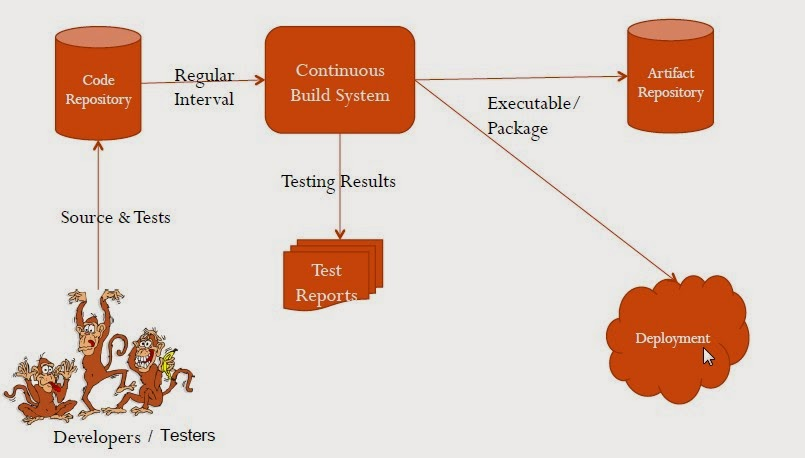
\includegraphics[width=10cm]{Workflow.jpg}
\caption{Continuous Integration Workflow}
\end{figure}

From Figure 1, some of the functions Jenkins provides are highlighted like generating testing reports, pushing to artifacts repositories, deploying to production or testing environments. Jenkins processes respond to GitHub commits. Section 4.4 will discuss how Jenkins is Setup. \\

Docker gives us functionality to create containers that can virtual run anywhere. To make this possible, Docker employs the concept of \emph{Docker images}, which are read-only executable binary files that contains the application software installed, configured and tested \cite{carl15}. Docker images are created by \emph{Dockerfiles}, which are simple scripts, similar to Makefile \citep{makefile}, developed using DevOps approach that defines software dependencies, environment variables etc... needed to execute the application. A sample Dockerfile will look like Figure 2. These are store created on Github.
\begin{figure}[!hb]
\centering
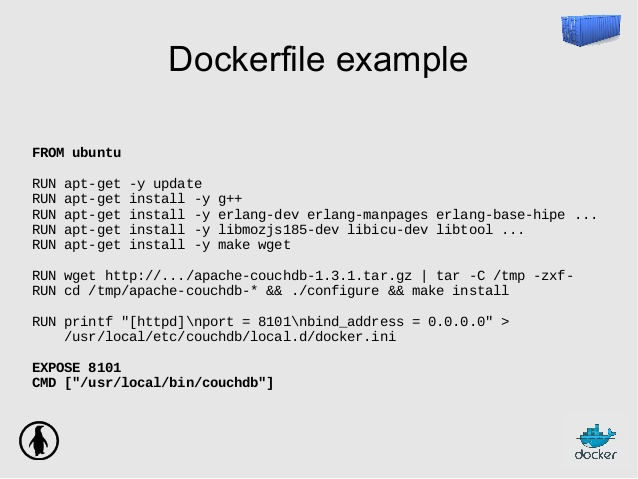
\includegraphics[width=10cm]{Dockerfile.jpg}
\caption{Sample Dockerfile}
\end{figure}

The beauty of Docker is the flexibility we can configure. Docker images can be created from Dockerfiles using Ansible \citep{ansible}, a provisioning, configuration management, application deployment tool. SAGrid has already began using Ansible for some of their installations, and this project will further continue exploring the feasibility of en-cooperating it. \\

Moving on to technologies the project will use for repositories, GitHub has already been mentioned as a code repository. Because its a known, common platform and has obvious advantages like social coding (Transparency and Collaboration) \citep{dabbish12}, we won't further discuss it here. The second repository for storing artifacts is called CernVM-FS \citep{cvmfs}. \\

Once applications are ported or certified or tested successfully, CVMFS makes sure they are available to as many grid sites as possible, on compute nodes where application execution takes place. CVMFS is designed not to be distinguishable from real file-system, file integrity is checked by every client compute node on every file and uses http protocol to make it mountable virtually anywhere. This also implies that CVMFS is designed with a caching system. Since grid sites are distributed, there exist a Distributed Hash Table algorithms to ensure a distributed caching system. Basically compute nodes decide based on their load if they keep files so they can serve them quickly. These cached files are available to other compute nodes within a grid site instead of the primary node. This makes CernVM-FS to out perform NFS and Lustre filesystem. For an in depth study, refer to \citep{blomer12} Another important fact to note is, executing these applications only require read-only access permissions, making the traffic between compute nodes are CVMFS repositories less congested. All computation output are written on local hard disks. Other technologies are used to send that data back to the user, but the focus of that is not for this paper. 


% Massively-parallel applications (such as GADGET), 
% self-contained applications (user-provided code),
% applications with complex dependency trees (such as Quantum Espresso), 
% and applications based on
% common frameworks (python or R applications).
\subsection{Scientific Applications}

\begin{description}
\item[GADGET] is a freely available code for cosmological N-body/SPH simulations on massively parallel computers with distributed memory. GADGET uses an explicit communication model that is implemented with the standardized MPI communication interface. This application is self-contained, with small add-on options like GSL and FFTW for added functionality. 

\item[Quantum Espresso] is an integrated suite of Open-Source computer codes for electronic-structure calculations and materials modeling at the nanoscale. It is based on density-functional theory, plane waves, and pseudo potentials. Refer to \citep{Qespresso} for more information. Quantum Espresso requires a fortran-95 compiler, a machine type (serial or parallel), MPI Libraries, BLAS, Lapack etc ... These variables might not be present or configured differently which causes the installation to fail.  

\item[R] is a language and environment for statistical computing and graphics. It provides a wide variety of statistical (linear and nonlinear modeling, classical statistical tests, time-series analysis, classification, clustering, …) and graphical techniques, and is highly extensible. Refer to \citep{R} for more information. These applications represents a wide variety of applications Grid scientists are working on.
\end{description} 

\subsection{Work Detail}
The work force that this project will require is the following:
Installations of the software platforms. There exists a SAGrid Jenkins platforms http://ci.sagrid.ac.za:8080/. What is needed is to write configuration of Jenkins jobs necessary to build tests. Setting up a Jenkins job  consists of the following elements \begin{enumerate*}[label=\itshape\alph*\upshape)]
\item configure a source version control with the job, where all the source code resides. This is GitHub repository.
\item configure triggers to control when Jenkins will perform builds. Whenever there is \emph{git commit}, automatic build will be triggered. 
\item configure the scripts that actually does the builds. The are usually shell or bash scripts.
\item configure the repository that will hold the builds results (artifacts). CVMFS comes into play.
\item configure notification via email or issue tracker to collaborators with the build results.
\end{enumerate*} 
Jenkins job configuration after these steps is done. \\

Next is Docker installation. Docker is available from online repositories (Docker or third-party) and simple to install, especially Using Yellowdog Updater, Modified (yum).  A server (virtual machine or physical) is required for this installation since SAGrid doesn't have an existing docker installation. A cluster of nodes will be provided for Docker and slave testing from the SAGrid cluster. SSH and HTTP access will be configured securely for public access to enable demonstrations publicly (especially for WITS). The docker plugin will be configured next which takes over the provisioning of applications to Jenkins slaves (desired hosts).  \\

CVMFS: \\

A number of scientific applications, mentioned on section 4.3 will be installed on this system. For each application, there will be Jenkins jobs created, dockerfiles created, docker images which are stored and finally executed on Grid sites through CVMFS. Scientific jobs will be executed and results verified by scientist working on the respected fields. 

% Presented Clearly And Well Organized
% Enough Collected To Test Hypothesis Or Answer Questions
% Student Understands Results (Discussion)
% Student Has Related Results To Research Hypothesis/Question
% Student Has Discussed Limitation(s) Of Own Research
% Student Has Placed Own Work Into Context With Other Research
% Student Has Discussed Own Level Of Contribution

% It is expected that these case studies will lead to insights necessary 
% to provide best-practice guidelines to future development and operation of the service, 
% especially related to optimisation and automation procedures.

% A practical working system is also expected.
\section{Results}
Expected Results \\
Link the expected results to the Research AIM (The questions)

% It Provides A Summary Of The Major Points Of The Proposal
% It Does Summarize The Document
% It Brings Together The Main Points
% It Highlights Most Important Results
% It Makes Clear Student’s Own Contribution
% Some Ideas For Future Work Presented
% Some Discussion Of Other Ways Of Addressing The Same Problem
\section{Conclusion}
Summary of the proposal \\
Highlight important points  - Bring it all together\\
What will not be covered and Future work \\

\bibliography{annot2}

\end{document}